\documentclass[10pt,a4paper]{article}



% Basic packages only
\usepackage[top=0.2in, bottom=0.2in, left=0.5in, right=0.5in]{geometry}
\usepackage{enumitem}
\usepackage{titlesec}
\usepackage{graphicx}
\usepackage{multicol}
\usepackage{tikz}
\usepackage{tabularx}
\usepackage{array}
\usepackage{fontawesome5}
\usepackage{xcolor}
\usepackage{pagecolor}
\usepackage{fontspec}
\usepackage{microtype}
\usepackage{amsmath}
\usepackage{xparse}


% Custom colors
\definecolor{bgcolor_color}{HTML}{423b28}
\definecolor{name_color}{HTML}{b9ad8c}
\definecolor{surname_color}{HTML}{877952}
\definecolor{title_color}{HTML}{b9ad8c}
\definecolor{blocktitle1_color}{HTML}{93d07c}
\definecolor{blocktitle2_color}{HTML}{669793}
\definecolor{blocktext1_color}{HTML}{B6E1E7}
\definecolor{blocktext2_color}{HTML}{3a7688}
\definecolor{linkcolor}{HTML}{43bbba}
\definecolor{skilltitle_color}{HTML}{93d07b}
\definecolor{filled_circle}{HTML}{d3cbb6}
\definecolor{empty_circle}{HTML}{887952}
\definecolor{dimmed}{HTML}{877952}


\usepackage[colorlinks=true, linkcolor=linkcolor, urlcolor=linkcolor]{hyperref}
\newfontfamily\cambria{cambriab.ttf}[Path=fonts/]
\setmainfont{calibri.ttf}[Path=fonts/]

\titleformat{\section}
  {\normalfont\Large\bfseries\centering} % font size, bold, centered
  {} % no section number
  {0pt} % no extra spacing between label and title
  {} % what to insert before the title

\pagecolor{bgcolor_color} % sets full background
\color{blocktext1_color}

\newcommand{\sectionline}[1]{%
  \vspace{0.5em}
  \begin{center}
    \textcolor{title_color}{\rule[0.5ex]{0.25\linewidth}{0.5pt}}
    ~{\LARGE \bfseries \textcolor{title_color}{\cambria #1}}~
    \textcolor{title_color}{\rule[0.5ex]{0.25\linewidth}{0.5pt}}
  \end{center}
  \vspace{0.05em}
}


\ExplSyntaxOn
\NewDocumentCommand{\circles}{mm}
 {
  \prg_replicate:nn { #1 } { \textcolor{filled_circle}{\large ●} }
  \prg_replicate:nn { \int_eval:n { #2 - #1 } } { \textcolor{empty_circle}{\large ●} }
 }
\ExplSyntaxOff

\titlespacing*{\section}{0pt}{0.8em}{0.4em}
\setlist[itemize]{topsep=0pt, partopsep=0pt, itemsep=2pt, parsep=0pt}


\begin{document}

% Header
\vspace{-3em}
\noindent
\makebox[\textwidth][t]{%

% Column 1: Image
\begin{minipage}[c]{0.3\textwidth}
  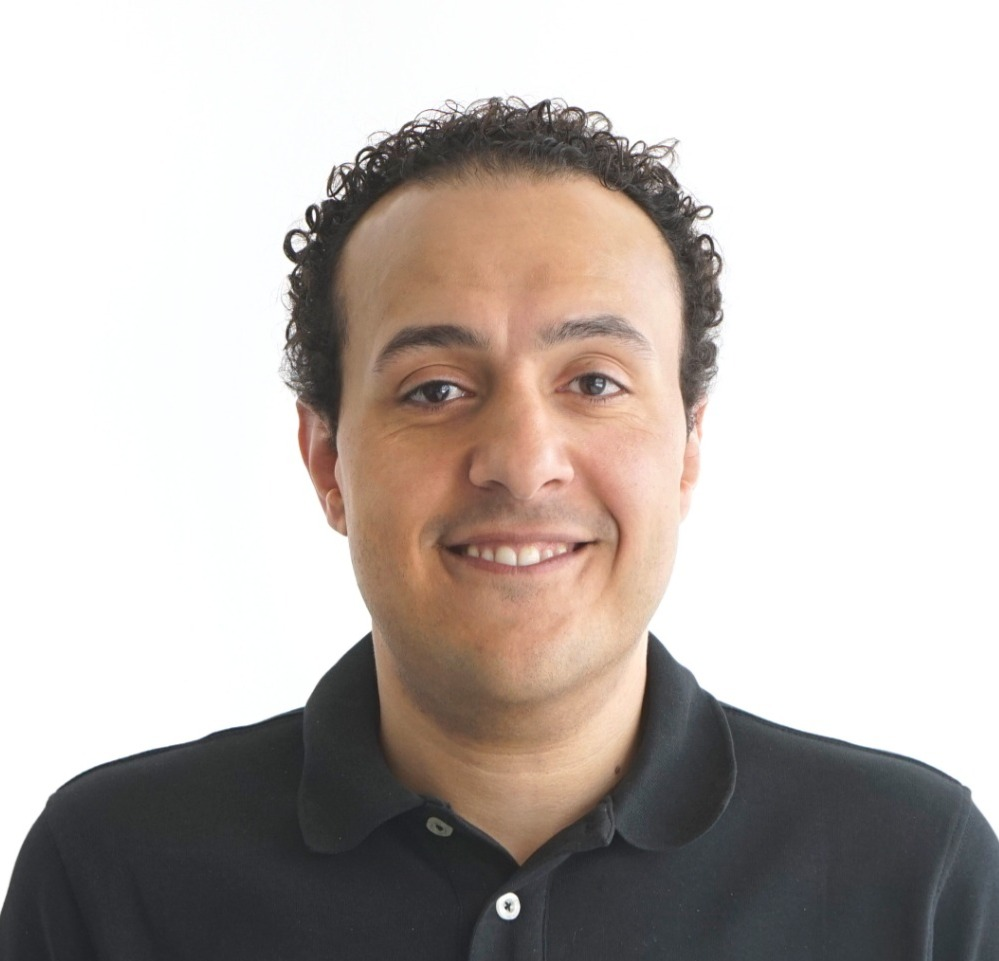
\includegraphics[width=0.8\linewidth]{images/my_image.jpg}
\end{minipage}%
\hspace{1em}

% Column 2: Name Block (baseline centered)
\begin{minipage}[c]{0.35\textwidth}
  {\fontsize{30pt}{32pt}\selectfont \textbf{\textcolor{name_color}{Amr}}}\\\\[-0.4em]
  \hspace{2.5em}{\fontsize{20pt}{22pt}\selectfont \textcolor{surname_color}{Aboughazala}}\\[0.8em]
\end{minipage}%
\hfill

% Column 3: Contact Info (forced to align at top)
\begin{minipage}[t]{0.35\textwidth}
  \begin{flushright}
    \textcolor{name_color}{\faEnvelope }\textcolor{linkcolor}{~\href{mailto:amr.abughazala@gmail.com}{amr.abughazala@gmail.com}}\\
    \textcolor{name_color}{\faPhone~+49 174 5969 482} \\
    \textcolor{name_color}{\faHome~Wieland Straße, Ulm, 89073} \\[1.5em]
    
    \textcolor{linkcolor}{\href{https://www.linkedin.com/in/amr-a-063776157/}{LinkedIn}} \quad
    \textcolor{linkcolor}{\href{https://www.xing.com/profile/Amr_Aboughazala/cv}{Xing}} \quad
    \textcolor{linkcolor}{\href{https://amr-aboughazala.super.site/}{Portfolio Site}}
  \end{flushright}
\end{minipage}%
}


% Objective
\sectionline{Objective}
\textcolor{blocktext1_color}{Bringing deep experience in R\&D and algorithm development, I aim to contribute to impactful work in signal processing, machine learning, perception, and computer vision within a research-focused environment.}

                      %% ---------------- R&D ---------------- %%
\sectionline{Key R\&D Contributions}

                         % ------ Doppler Ambiguity Head ------ %
                         
\begin{tabular}{@{}m{0.5cm}@{\hspace{0.5em}}m{2.2cm}@{\hspace{0.5em}}m{15cm}@{}}
  \raisebox{1.3em}{
\includegraphics[width=0.9cm]{images/scantinel_logo.png}} & 
  \raisebox{1.8em}{\begin{minipage}[t]{\linewidth}
  \centering
    \textcolor{blocktitle1_color}{Sep. 21}\\
    \textcolor{blocktitle1_color}{Present}
  \end{minipage} 
  } &
  \raisebox{0.5em}{\begin{minipage}[t]{\linewidth}
    \raggedright
    {\fontsize{11pt}{9pt}\selectfont\textbf{\textcolor{blocktitle1_color}{\text{Lidar Doppler Ambiguity,}}}}
    {\fontsize{9pt}{9pt}\selectfont\textcolor{blocktitle2_color}{Scantinel Photonics GmbH, Ulm Germany}}
  \end{minipage}}
\end{tabular}

                         % ------ Doppler Ambiguity Body ------ %
                         
\vspace{-1em}
\begin{itemize}[leftmargin=*]
  \item Responsible of R\&D, implementation, testing and enhancing of a novel algorithm for Doppler ambiguity in FMCW LiDAR systems.
  \\ {\fontsize{10pt}{10pt}\selectfont\textcolor{blocktext2_color}{{\fontsize{10pt}{10pt}\selectfont\textcolor{blocktext2_color}{\href{https://amr-aboughazala.super.site/doppler-ambiguity-solution}{Sources}}}: VQRV, VTRV, VQR}}
  

\end{itemize}


                            % ------ Perception Head ------ %
                         
\vspace{1em}                       
\begin{tabular}{@{}m{0.5cm}@{\hspace{0.5em}}m{2.2cm}@{\hspace{0.5em}}m{15cm}@{}}
  \raisebox{1.3em}{
\includegraphics[width=0.9cm]{images/scantinel_logo.png}} & 
  \raisebox{1.8em}{\begin{minipage}[t]{\linewidth}
  \centering
    \textcolor{blocktitle1_color}{Sep. 21}\\
    \textcolor{blocktitle1_color}{Sep. 22}
  \end{minipage} 
  } &
  \raisebox{0.5em}{\begin{minipage}[t]{\linewidth}
    \raggedright
    {\fontsize{11pt}{9pt}\selectfont\textbf{\textcolor{blocktitle1_color}{\text{Perception,}}}}
    {\fontsize{9pt}{9pt}\selectfont\textcolor{blocktitle2_color}{Scantinel Photonics GmbH, Ulm Germany}}
  \end{minipage}}
\end{tabular}


                           % ------ Perception Body  ------ %
\vspace{-1em}
\begin{itemize}[leftmargin=*]
  \item Proposed and implemented an internal perception pipeline (filtering, segmentation, object detection, tracking).\\ {\fontsize{10pt}{10pt}\selectfont\textcolor{blocktext2_color}{Sources: Ransac, knn, kd-tree, JPDA Tracking}}. 
  \item Designed novel filters improving performance from 450 ms to 30 ms 
  \\ {\fontsize{10pt}{10pt}\selectfont\textcolor{blocktext2_color}{{\fontsize{10pt}{10pt}\selectfont\textcolor{blocktext2_color}{\href{https://amr-aboughazala.super.site/data-analysis}{Sources}}}: Dense Cluster Filter “DCL” and the Multilevel Neighboring Filter “MLN”}}

\end{itemize}


                            % ------ Data Analysis Head ------ %           
\vspace{1.3em}                       
\begin{tabular}{@{}m{0.5cm}@{\hspace{0.5em}}m{2.2cm}@{\hspace{0.5em}}m{15cm}@{}}
  \raisebox{-0.5em}{
\includegraphics[width=0.9cm]{images/scantinel_logo.png}} & 
  \raisebox{1em}{\begin{minipage}[t]{\linewidth}
  \centering
    \textcolor{blocktitle1_color}{Jun. 23}\\
    \textcolor{blocktitle1_color}{Oct. 23}
  \end{minipage} 
  } &
  \raisebox{0.5em}{\begin{minipage}[t]{\linewidth}
    \raggedright
    {\fontsize{11pt}{9pt}\selectfont\textbf{\textcolor{blocktitle1_color}{\text{Time–Frequency Signal Analysis and Comparative Evaluation of Detection Methods,}}}}
    {\fontsize{9pt}{9pt}\selectfont\textcolor{blocktitle2_color}{Scantinel Photonics GmbH, Ulm Germany}}
  \end{minipage}}
\end{tabular}


                           % ------ Data Analysis Body  ------ %
                         
\vspace{1em}
\begin{itemize}[leftmargin=*]
  \item Implemented and applied classical windowing and detection methods on raw signal data to evaluate detection reliability, supported by statistical analysis. 
  \\ {\fontsize{10pt}{10pt}\selectfont\textcolor{blocktext2_color}{\href{https://amr-aboughazala.super.site/data-analysis}{Sources}: Windows (Hann, Chebyshev, Planck-Taper), Peak Detection: (CA-CFAR, OS-CFAR, RANSAC, M-estimator)}}
  \item Simulated a dual-signal FFT technique real/imaginary packing to enable simultaneous processing.
\end{itemize}



                              % ------ Navimatix Head ------ %
\vspace{1em}
\begin{tabular}{@{}m{0.5cm}@{\hspace{0.5em}}m{2.2cm}@{\hspace{0.5em}}m{15cm}@{}}
  \raisebox{1.3em}{
\includegraphics[width=0.9cm]{images/navi2_logo.png}} & 
  \raisebox{1.8em}{\begin{minipage}[t]{\linewidth}
  \centering
    \textcolor{blocktitle1_color}{Jan. 19}\\
    \textcolor{blocktitle1_color}{Jul. 21}
  \end{minipage} 
  } &
  \raisebox{0.5em}{\begin{minipage}[t]{\linewidth}
    \raggedright
    {\fontsize{11pt}{9pt}\selectfont\textbf{\textcolor{blocktitle1_color}{\text{Automated Image Analysis for Segmenting Bacteria,}}}}
    {\fontsize{9pt}{9pt}\selectfont\textcolor{blocktitle2_color}{Navimatix GmbH, Jena Germany}}
  \end{minipage}}
\end{tabular}


                                 % ------ Navimatix Block ------ %
\vspace{-1em}
\begin{itemize}[leftmargin=*]
  \item A full pipeline image processing algorithms for bacteria counting on Fluorescence Images.\\ {\fontsize{10pt}{10pt}\selectfont\textcolor{blocktext2_color}{\fontsize{10pt}{10pt}\selectfont\textcolor{blocktext2_color}{Sources: Median Filter, ISODATA Segmentation, Opening Filter, 2D \& 3D counting}}}
\end{itemize}

                          

                             % ------ Master Thesis Head ------ %

\vspace{1em}
\begin{tabular}{@{}m{0.5cm}@{\hspace{0.5em}}m{2.2cm}@{\hspace{0.5em}}m{15cm}@{}}
\raisebox{1.3em}{
\includegraphics[width=0.9cm]{images/ilmenau1_logo.png}} & 
  \raisebox{1.8em}{\begin{minipage}[t]{\linewidth}
  \centering
    \textcolor{blocktitle1_color}{Mar. 17}\\
    \textcolor{blocktitle1_color}{Feb. 18}
  \end{minipage} 
  } &
  \raisebox{0.5em}{\begin{minipage}[t]{\linewidth}
    \raggedright
    {\fontsize{11pt}{9pt}\selectfont\textbf{\textcolor{blocktitle1_color}{\text{Positivity Decomposition Algorithms on EEG/MEG Data,}}}}
    {\fontsize{9pt}{9pt}\selectfont\textcolor{blocktitle2_color}{Master Thesis, MSCSP Group, TU Ilmenau}}
  \end{minipage}}
\end{tabular}                               

                                % ------ Master Thesis Block ------ %
\vspace{-1em}
\begin{itemize}[leftmargin=*]
  \item Implemented non-negativity constraints on tensor-based blind source separation algorithm 
  \\ {\fontsize{10pt}{10pt}\selectfont\textcolor{blocktext2_color}{Sources: {\fontsize{10pt}{10pt}\selectfont\textcolor{blocktext2_color}{\href{https://ieeexplore.ieee.org/document/8313193}{Publication}}, {\fontsize{10pt}{10pt}\selectfont\textcolor{blocktext2_color}{\href{https://amr-aboughazala.super.site/non-negative-semi-algebraic-cp-decomposition-via-simultaneous-matrix-diagonalization}{Thesis Publication (not completed)}}}}}}
\end{itemize}


                             % ------ Advanced Research Head ------ %
\vspace{1.3em}
\begin{tabular}{@{}m{0.5cm}@{\hspace{0.5em}}m{2.2cm}@{\hspace{0.5em}}m{15cm}@{}}
  \raisebox{-0.5em}{
\includegraphics[width=0.9cm]{images/ilmenau1_logo.png}} & 
  \raisebox{0.3em}{\begin{minipage}[t]{\linewidth}
  \centering
    \textcolor{blocktitle1_color}{Sep. 16}\\
    \textcolor{blocktitle1_color}{Feb. 17}
  \end{minipage} 
  } &
  \raisebox{0.5em}{\begin{minipage}[t]{\linewidth}
    \raggedright
    {\fontsize{11pt}{9pt}\selectfont\textbf{\textcolor{blocktitle1_color}{\text{Decomposition of a Low Rank Tensor with Missing Entries,}}}}
    {\fontsize{9pt}{9pt}\selectfont\textcolor{blocktitle2_color}{Advanced Research Project, MSCSP Group, TU Ilmenau}}
  \end{minipage}}
\end{tabular}                                  

                                % ------ Advanced Research Block ------ %
\vspace{0.4em}
\begin{itemize}[leftmargin=*]
  \item Developed a missing imputation tensor algorithm to make it adaptive as per step size and rank estimation.
  \\ {\fontsize{10pt}{10pt}\selectfont\textcolor{blocktext2_color}{\href{https://amr-aboughazala.super.site/decomposition-of-a-low-rank-tensor-with-missing-entries}{Sources}}}       
\end{itemize}              

                        


                      %% ---------------- Technical Skills ---------------- %%     
\sectionline{Technical Skills}
\hspace*{-0.1em}  % try -1em or adjust as needed
\noindent\makebox[\textwidth][c]{%
\begin{minipage}[t]{0.2\textwidth}
\begin{center}
\textbf{{\fontsize{10pt}{10pt}\selectfont\textcolor{skilltitle_color}{Languages}}} \\[0.5em]
\begin{tabular}{@{}l l@{}}
Matlab & \circles{6}{6}\\
Python & \circles{6}{6}\\
C++ & \circles{3}{6}\\
Java & \circles{3}{6}\\
C\# & \circles{3}{6}
\end{tabular}
\end{center}
\end{minipage}%
\hspace{1em}
\begin{minipage}[t]{0.65\textwidth}
  \begin{center}
  \textbf{{\fontsize{10pt}{10pt}\selectfont\textcolor{skilltitle_color}{Libraries}}}
  \end{center}
  \begin{minipage}[t]{0.4\textwidth}
    \textbf{DATA:} numpy, pandas, scipy\\
    \textbf{PLOT:} matplotlib, plotly, pyqtgraph\\
    \textbf{ML:} pytorch, scikit-learn, spconv\\
    \textbf{CV:} opencv
  \end{minipage}%
  \hfill
  \begin{minipage}[t]{0.5\textwidth}
    \textbf{VC:} git, gitlab\\
    \textbf{GUI:} PyQt, JavaFX, WPF\\
    \textbf{OOP:} MVC, MVVM\\
    \textbf{LIDAR:} open3D, open3DML, pytorch3d
  \end{minipage}
\end{minipage}%
\hspace{1em}
\begin{minipage}[t]{0.22\textwidth}
  \begin{center}
  \textbf{{\fontsize{10pt}{10pt}\selectfont\textcolor{skilltitle_color}{Libraries}}} \\[0.5em]
  Signal Processing\\
  {\fontsize{10pt}{10pt}\selectfont\textcolor{blocktext2_color} {\href{https://math.stackexchange.com/users/282534/mour-ka}{Optimization-Mathematics}}}\\
  Machine Learning\\
  Wireless Communication\\
  Audio \& Image Processing\\
  Communication Networks
  \end{center}
\end{minipage}%
}

                      %% ---------------- Industry Experience ---------------- %%
                      
\newpage
\sectionline{Industry Experience}                    
                                    % ------ Scantinel Head ------ %                          
\begin{tabular}{@{}m{0.5cm}@{\hspace{0.5em}}m{2.2cm}@{\hspace{0.5em}}m{15cm}@{}}
  \raisebox{-0.5em}{
\includegraphics[width=0.9cm]{images/scantinel_logo.png}} & 
  \raisebox{0.3em}{\begin{minipage}[t]{\linewidth}
  \centering
    \textcolor{blocktitle1_color}{Sep. 21}\\
    \textcolor{blocktitle1_color}{Present}
  \end{minipage} 
  } &
  \raisebox{0.5em}{\begin{minipage}[t]{\linewidth}
    \raggedright
    {\fontsize{11pt}{9pt}\selectfont\textbf{\textcolor{blocktitle1_color}{\text{Senior Algorithm and Data Processing Developer,}}}}
    {\fontsize{9pt}{9pt}\selectfont\textcolor{blocktitle2_color}{Scantinel Photonics GmbH, Ulm Germany}}
  \end{minipage}}
\end{tabular}                                  

                                  % ------ Scantinel Block ------ %
\vspace{0.4em}
\begin{itemize}[leftmargin=*]
  \item Led the architecture of new system software, collaborating with embedded teams to align hardware/software interfaces. 
  \\ {\fontsize{10pt}{10pt}\selectfont\textcolor{blocktext2_color}{Skills: Pattern design MVC/MVVM }}    

  \item  Developed and maintained real-time and offline visualization GUIs supporting continuous feature development and release cycles for internal users and customers over two years. 
  \\ {\fontsize{10pt}{10pt}\selectfont\textcolor{blocktext2_color}{Skills: python, PyQt}}     
  
  \item Developed a user-facing GUI integrating multiple signal processing algorithms and visualization tools, enabling interactive analysis and testing across devices with real-time performance evaluation.
  
  \item implementing testing development creating unit, integration and functional testing. 
  \\ {\fontsize{10pt}{10pt}\selectfont\textcolor{blocktext2_color}{Skills: pytest}}  
\end{itemize}                
                
                                  % ------ Navimatix Head ------ %                 
\vspace{1em}                                  
\begin{tabular}{@{}m{0.5cm}@{\hspace{0.5em}}m{2.2cm}@{\hspace{0.5em}}m{15cm}@{}}
  \raisebox{1.3em}{
\includegraphics[width=0.9cm]{images/navi2_logo.png}} & 
  \raisebox{1.8em}{\begin{minipage}[t]{\linewidth}
  \centering
    \textcolor{blocktitle1_color}{Jan. 19}\\
    \textcolor{blocktitle1_color}{Jul. 21}
  \end{minipage} 
  } &
  \raisebox{0.5em}{\begin{minipage}[t]{\linewidth}
    \raggedright
    {\fontsize{11pt}{9pt}\selectfont\textbf{\textcolor{blocktitle1_color}{\text{Software Developer,}}}}
    {\fontsize{9pt}{9pt}\selectfont\textcolor{blocktitle2_color}{Navimatix GmbH, Jena Germany}}
  \end{minipage}}
\end{tabular}    

                           % ------ Navimatix Block ------ %
\vspace{-1em}
\begin{itemize}[leftmargin=*]
  \item Developed a GUI applying image processing algorithm on Microscopic Images to count bacteria.
  \item Implemented several user interface applications. 
  \\ {\fontsize{10pt}{10pt}\selectfont\textcolor{blocktext2_color}{Skills: JavaFX, .Net Framework WPF and Delphi.}}  
\end{itemize} 


                             % ------ OBDient Head ------ %               
\vspace{0.5em}
\begin{tabular}{@{}m{0.5cm}@{\hspace{0.5em}}m{2.2cm}@{\hspace{0.5em}}m{15cm}@{}}
  \raisebox{1.3em}{
\includegraphics[width=0.9cm]{images/ilmenau1_logo.png}} & 
  \raisebox{1.8em}{\begin{minipage}[t]{\linewidth}
  \centering
    \textcolor{blocktitle1_color}{Jul. 18}\\
    \textcolor{blocktitle1_color}{Nov. 18}
  \end{minipage} 
  } &
  \raisebox{0.5em}{\begin{minipage}[t]{\linewidth}
    \raggedright
    {\fontsize{11pt}{9pt}\selectfont\textbf{\textcolor{blocktitle1_color}{\text{Founding Engineer,}}}}
    {\fontsize{9pt}{9pt}\selectfont\textcolor{blocktitle2_color}{Start Up OBDient, TU Ilmenau}}
  \end{minipage}}
\end{tabular}                             

                               % ------ OBDient Block ------ %             
\vspace{-1em}
\begin{itemize}[leftmargin=*]
  \item  Implemented data sensor fusion using GPS and Accelerometer on Raspberry Pi.  
  \\ {\fontsize{10pt}{10pt}\selectfont\textcolor{blocktext2_color}{Tools: NMEA Data of a NEO-6M GPS, MPU6050 GyroSensor, Raspberry Pi 3 B+}}
  \item Implemented Kalman Filter GPS reception using a motion model of vehicles and pedestrians.
\end{itemize}                               

                             % ------ Siemens Head ------ %
\vspace{1.3em}
\begin{tabular}{@{}m{0.5cm}@{\hspace{0.5em}}m{2.2cm}@{\hspace{0.5em}}m{15cm}@{}}
  \raisebox{-0.3em}{
\includegraphics[width=0.9cm]{images/siemens4_logo.jpg}} & 
  \raisebox{1em}{\begin{minipage}[t]{\linewidth}
  \centering
    \textcolor{blocktitle1_color}{Sep. 16}\\
    \textcolor{blocktitle1_color}{Feb. 17}
  \end{minipage} 
  } &
  \raisebox{0.5em}{\begin{minipage}[t]{\linewidth}
    \raggedright
    {\fontsize{11pt}{9pt}\selectfont\textbf{\textcolor{blocktitle1_color}{\text{Working Student,}}}}
    {\fontsize{9pt}{9pt}\selectfont\textcolor{blocktitle2_color}{Siemens, Network R\&D, Munich Germany}}
  \end{minipage}}
\end{tabular}                                

                                 % ------ Siemens Block ------ %
\vspace{0.4em}
\begin{itemize}[leftmargin=*]
  \item Implemented a simulation of TSN Scheduler as well as converter from SDN controller using C++.\\ {\fontsize{10pt}{10pt}\selectfont\textcolor{blocktext2_color}{\fontsize{10pt}{10pt}\selectfont\textcolor{blocktext2_color}{Sources: C++, Omnet++, }}} {\fontsize{10pt}{10pt}\selectfont\textcolor{blocktext2_color}{\href{https://1.ieee802.org/tsn/}{Time Sensitive Network for Industry v.4}}}.       
\end{itemize}    


                             % ------ Orange Head ------ %
\vspace{1.3em}
\begin{tabular}{@{}m{0.5cm}@{\hspace{0.5em}}m{2.2cm}@{\hspace{0.5em}}m{15cm}@{}}
  \raisebox{-0.3em}{
\includegraphics[width=0.9cm]{images/orange_logo.jpg}} & 
  \raisebox{1em}{\begin{minipage}[t]{\linewidth}
  \centering
    \textcolor{blocktitle1_color}{Jul. 11}\\
    \textcolor{blocktitle1_color}{Aug. 14}
  \end{minipage} 
  } &
  \raisebox{0.5em}{\begin{minipage}[t]{\linewidth}
    \raggedright
    {\fontsize{11pt}{9pt}\selectfont\textbf{\textcolor{blocktitle1_color}{\text{Customer Technical Network Specialist,}}}}
    {\fontsize{9pt}{9pt}\selectfont\textcolor{blocktitle2_color}{Orange Business Services, Cairo Egypt}}
  \end{minipage}}
\end{tabular} 


                                 % ------ Orange Block ------ %
\vspace{0.4em}
\begin{itemize}[leftmargin=*]
  \item Diagnose WAN network fault-related cases both proactive and reactive being responsible of the faults to resolution.
  \item Shift Leader for a group of 5 to 10 daily, managing the workflow through the team. 
\end{itemize}

% Education
\sectionline{Education}
\textbf{M.Sc. in Communications and Signal Processing}\\
Technische Universität Ilmenau, Germany\\
\textit{Sep 2014 -- Feb 2018}\\
Major: Mobile Communications, Adaptive Arrays, DSP\\
Grade: 2.2/1.0

\vspace{0.6em}
\textbf{B.Sc. in Electronics and Communication}\\
Arab Academy for Science and Technology, Alexandria\\
\textit{Sep 2007 -- Feb 2010}\\
Grade: 1.3/1.0 — Top of class

% Courses
\sectionline{Certificates and Online Courses}
\begin{itemize}[leftmargin=*]
  \item 22 May 2019: \href{https://www.udemy.com/certificate/UC-XN2ILPOB/}{OOP in Java — Udemy}
  \item 24 Aug. 2020: \href{https://coursera.org/share/e32b80d8e0b32b48e4ad6fe40cea746e}{Machine Learning — Coursera}
  \item 14 May 2021: \href{https://coursera.org/share/15d74342746d2872a09dcc5a75ff460c}{Structuring ML Projects — Coursera}
  \item 30 Apr. 2021: \href{https://coursera.org/share/0ca157f56b99f56122ab247589555837}{Neural Networks and Deep Learning — Coursera}
  \item 04 Jun. 2021: \href{https://coursera.org/share/e0bd7b6ea301e1108dfe609c783f2706}{Convolutional Neural Networks — Coursera}
  \item 07 May 2021: \href{https://coursera.org/share/ef6671ff524b9d2e5c1e0e282d457f56}{Improving DNN Hyperparameter Tuning, Regularization and Optimization — Coursera}
  \item 24 Aug. 2021: \href{http://www.udacity.com/certificate/e/95ce8498-c21f-11eb-aa1a-5f098308d726}{Sensor Fusion — Udacity (Mercedes Benz)}
\end{itemize}


\vspace{2em}
\sectionline{Personal Skills}

\begin{center}
\begin{minipage}[t]{0.45\textwidth}
  \centering
  \textbf{{\fontsize{12pt}{12pt}\selectfont\textcolor{skilltitle_color}{Languages}}} \\[0.5em]
  {\fontsize{10pt}{10pt}\selectfont Arabic:} {\fontsize{10pt}{10pt}\selectfont\textcolor{dimmed}{Native}} \\
{\fontsize{10pt}{10pt}\selectfont English:} {\fontsize{10pt}{10pt}\selectfont\textcolor{dimmed}{Fluent}} \\
{\fontsize{10pt}{10pt}\selectfont German:} {\fontsize{10pt}{10pt}\selectfont\textcolor{dimmed}{B1 TELC}} \\
    {\footnotesize
    \begin{tabular}{@{}l l@{}}
    \selectfont\textcolor{dimmed}{Hören} & \circles{2}{6}\\
    \selectfont\textcolor{dimmed}{Lesen} & \circles{2}{6}\\
    \selectfont\textcolor{dimmed}{Schreiben} & \circles{2}{6}\\
    \selectfont\textcolor{dimmed}{Sprechen} & \circles{2}{6}\\
    \end{tabular}
    }
    


\end{minipage}%
\hfill
\begin{minipage}[t]{0.45\textwidth}
  \begin{center}
  \textbf{{\fontsize{12pt}{12pt}\selectfont\textcolor{skilltitle_color}{Interests}}} \\[0.5em]
  \begin{tabular}{@{}l l@{}}
  \fontsize{10pt}{10pt}{Graphics Design}\\
  \fontsize{10pt}{10pt}{Tennis}\\
  \fontsize{10pt}{10pt}{Movies and TV Series}\\
  \fontsize{10pt}{10pt}{Trying Different Restaurants}\\
  \end{tabular}
\end{center}
\end{minipage}
\end{center}




\end{document}